\documentclass[tikz,border=10pt]{standalone}
\usepackage{tikz}
\usetikzlibrary{shapes.misc, arrows.meta, positioning, fit, backgrounds}

\begin{document}
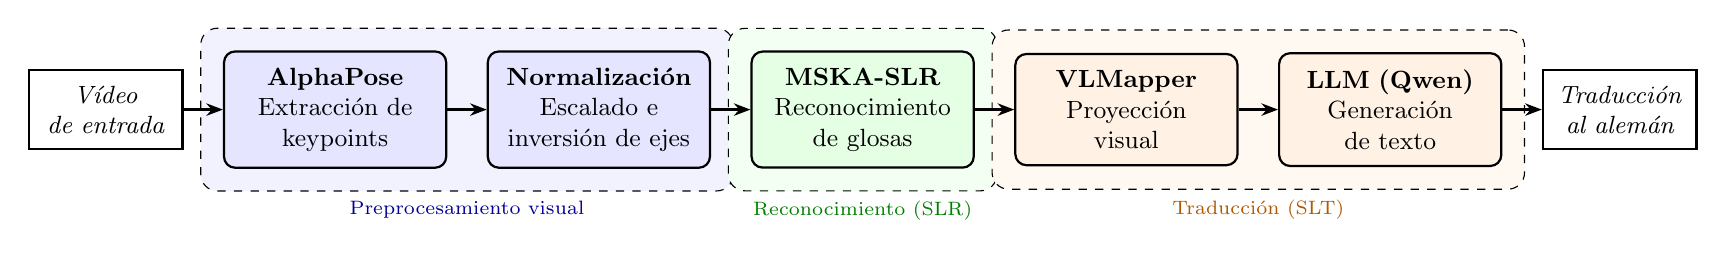
\begin{tikzpicture}[
    node distance = 0.6cm and 0.5cm,
    box/.style = {
        rounded corners=4pt,
        draw,
        thick,
        align=center,
        font=\small,
        minimum height=1.1cm,
        text width=2.4cm,
        inner sep=6pt
    },
    io/.style = {
        draw,
        thick,
        align=center,
        font=\small\itshape,
        minimum height=1.0cm,
        text width=1.6cm,
        inner sep=5pt
    },
    arrow/.style = {-{Stealth[length=6pt]}, thick},
    group/.style = {
        rounded corners=6pt,
        draw,
        dashed,
        inner sep=8pt
    }
]

%% ── Nodos ──────────────────────────────────────────────────────────────────

\node[io] (video) {Vídeo\\de entrada};

\node[box, fill=blue!10,  right=of video]  (alpha)  {\textbf{AlphaPose}\\Extracción de\\keypoints};

\node[box, fill=blue!10,  right=of alpha]  (norm)   {\textbf{Normalización}\\Escalado e\\inversión de ejes};

\node[box, fill=green!10, right=of norm]   (mska)   {\textbf{MSKA-SLR}\\Reconocimiento\\de glosas};

\node[box, fill=orange!10,right=of mska]   (vlmap)  {\textbf{VLMapper}\\Proyección\\visual};

\node[box, fill=orange!10,right=of vlmap]  (llm)    {\textbf{LLM (Qwen)}\\Generación\\de texto};

\node[io,  right=of llm]  (out)    {Traducción\\al alemán};

%% ── Flechas ─────────────────────────────────────────────────────────────────

\draw[arrow] (video)  -- (alpha);
\draw[arrow] (alpha)  -- (norm);
\draw[arrow] (norm)   -- (mska);
\draw[arrow] (mska)   -- (vlmap);
\draw[arrow] (vlmap)  -- (llm);
\draw[arrow] (llm)    -- (out);

%% ── Etiqueta intermedia en flecha MSKA → VLMapper ──────────────────────────

\node[font=\scriptsize\itshape, above=0.08cm of vlmap.west, xshift=0.1cm]
    {};

%% ── Grupos de fases ─────────────────────────────────────────────────────────

% Fase 1: Preprocesamiento visual
\begin{scope}[on background layer]
    \node[group, fill=blue!5,
          fit=(alpha)(norm),
          label={[font=\scriptsize, blue!60!black]below:Preprocesamiento visual}]
          (grp1) {};
\end{scope}

% Fase 2: Reconocimiento
\begin{scope}[on background layer]
    \node[group, fill=green!5,
          fit=(mska),
          label={[font=\scriptsize, green!50!black]below:Reconocimiento (SLR)}]
          (grp2) {};
\end{scope}

% Fase 3: Traducción
\begin{scope}[on background layer]
    \node[group, fill=orange!5,
          fit=(vlmap)(llm),
          label={[font=\scriptsize, orange!70!black]below:Traducción (SLT)}]
          (grp3) {};
\end{scope}

\end{tikzpicture}
\end{document}
